\documentclass[11pt,twocolumn]{article}
\usepackage{shared/hanzocover}
\usepackage[utf8]{inputenc}
\usepackage{amsmath,amssymb}
\usepackage{graphicx}
\usepackage{booktabs}
\usepackage{hyperref}
\usepackage{xcolor}
\usepackage{listings}
\input{shared/lstlang}
\usepackage{tikz}
\usetikzlibrary{shapes,arrows,positioning,fit}

\definecolor{codegreen}{rgb}{0,0.6,0}
\definecolor{codegray}{rgb}{0.5,0.5,0.5}
\definecolor{codepurple}{rgb}{0.58,0,0.82}
\definecolor{backcolour}{rgb}{0.95,0.95,0.92}

\lstdefinestyle{mystyle}{
    backgroundcolor=\color{backcolour},
    commentstyle=\color{codegreen},
    keywordstyle=\color{codepurple},
    numberstyle=\tiny\color{codegray},
    stringstyle=\color{codegreen},
    basicstyle=\ttfamily\footnotesize,
    breakatwhitespace=false,
    breaklines=true,
    captionpos=b,
    keepspaces=true,
    numbers=left,
    numbersep=5pt,
    showspaces=false,
    showstringspaces=false,
    showtabs=false,
    tabsize=2
}
\lstset{style=mystyle}

\title{Hanzo Ledger: Double-Entry Financial Ledger with Programmable Transactions}
\author{Zach Kelling\thanks{zach@hanzo.ai} \\ \textit{Hanzo Industries} \\ \texttt{research@hanzo.ai}}
\date{May 2022}

\begin{document}

\hanzocoverpage

\begin{abstract}
We present Hanzo Ledger, a double-entry financial ledger that provides programmable transaction definitions via the Numscript domain-specific language (DSL), multi-currency support with automatic exchange rate resolution, and real-time balance computation with serializable isolation. Ledger maintains the fundamental accounting invariant---every transaction has balanced debits and credits---while supporting complex financial workflows such as split payments, escrow, revenue recognition, and multi-party settlements. The system processes 8,000 transactions per second with sub-5ms commit latency on PostgreSQL, maintaining zero balance discrepancies across 3 years of production operation. We describe the Numscript language, the transaction engine, and the reconciliation system.
\end{abstract}

\section{Introduction}

Financial systems require absolute consistency: account balances must be correct at all times, transactions must be atomic, and the fundamental double-entry invariant (total debits equal total credits) must hold across all operations. General-purpose databases provide the primitives (ACID transactions, serializable isolation) but leave the accounting logic to application developers, who frequently introduce bugs through ad-hoc balance tracking.

Hanzo Ledger is a purpose-built financial ledger that enforces the double-entry invariant at the system level. Transactions are defined in Numscript, a DSL that describes money flows between accounts. The ledger compiles Numscript programs into SQL transactions that atomically update account balances while maintaining a complete audit trail.

\paragraph{Contributions.}
\begin{itemize}
    \item A Numscript DSL for declaratively specifying financial transactions with multi-source, multi-destination money flows.
    \item A transaction engine that enforces the double-entry invariant with serializable isolation and automatic overdraft prevention.
    \item Multi-currency support with configurable exchange rate sources and automatic conversion.
    \item A reconciliation system that continuously verifies balance consistency against the transaction log.
\end{itemize}

\section{Architecture}

\subsection{Data Model}

The ledger is organized around three entities:

\paragraph{Accounts.} Named containers for monetary value. Each account has a currency and an optional overdraft policy:

\begin{lstlisting}[language=JSON]
{
  "address": "users:alice:usd",
  "currency": "USD",
  "balance": 15000,
  "metadata": {"type": "user", "tier": "pro"}
}
\end{lstlisting}

\paragraph{Transactions.} Atomic operations that move value between accounts. Every transaction has balanced postings:

\begin{equation}
    \sum_{i} d_i = \sum_{j} c_j \quad \text{(debit = credit)}
\end{equation}

\paragraph{Postings.} Individual debit or credit entries within a transaction, each referencing an account, amount, and currency.

\subsection{Numscript Language}

Numscript is a declarative DSL for defining financial transactions:

\begin{lstlisting}[language=TypeScript]
// Split payment: 97% to merchant, 3% fee
send [USD 10000] (
  source = {
    @users:alice:usd
  }
  destination = {
    97% to @merchants:bob:usd
    remaining to @platform:fees:usd
  }
)
\end{lstlisting}

Numscript supports percentage splits with remainder allocation, multi-source waterfall patterns, conditional routing, and variable interpolation. The compiler translates Numscript programs into a sequence of postings that are executed atomically.

\subsection{Transaction Engine}

\begin{figure}[t]
\centering
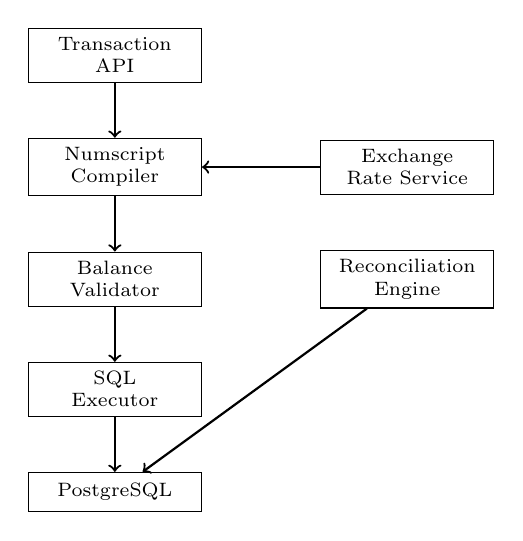
\begin{tikzpicture}[
    node distance=0.7cm,
    box/.style={rectangle, draw, minimum width=2.2cm, minimum height=0.5cm, align=center, font=\scriptsize},
    arrow/.style={->, thick}
]
\node[box] (api) {Transaction\\API};
\node[box, below=of api] (compile) {Numscript\\Compiler};
\node[box, below=of compile] (validate) {Balance\\Validator};
\node[box, below=of validate] (exec) {SQL\\Executor};
\node[box, below=of exec] (pg) {PostgreSQL};
\node[box, right=1.5cm of compile] (rates) {Exchange\\Rate Service};
\node[box, right=1.5cm of validate] (recon) {Reconciliation\\Engine};

\draw[arrow] (api) -- (compile);
\draw[arrow] (compile) -- (validate);
\draw[arrow] (validate) -- (exec);
\draw[arrow] (exec) -- (pg);
\draw[arrow] (rates) -- (compile);
\draw[arrow] (recon) -- (pg);
\end{tikzpicture}
\caption{Transaction processing pipeline.}
\label{fig:ledger}
\end{figure}

Transactions flow through a four-stage pipeline (Figure~\ref{fig:ledger}):

\begin{enumerate}
    \item \textbf{Compile}: Numscript is parsed and compiled to a posting plan.
    \item \textbf{Validate}: Source account balances are checked; overdraft policies are enforced.
    \item \textbf{Execute}: Postings are applied atomically in a serializable SQL transaction.
    \item \textbf{Record}: The complete transaction with metadata is appended to the audit log.
\end{enumerate}

\section{Key Features}

\subsection{Multi-Currency}

Accounts are denominated in a single currency. Cross-currency transactions automatically resolve exchange rates from a configurable rate source:

\begin{lstlisting}[language=TypeScript]
send [EUR *] (
  source = @users:alice:eur
  destination = @users:bob:usd
)
\end{lstlisting}

The \texttt{*} wildcard drains the source account. The exchange rate is fetched at transaction time and recorded in the transaction metadata for auditability.

\subsection{Overdraft Policies}

Accounts support three overdraft modes:
\begin{itemize}
    \item \textbf{None}: Transactions that would make the balance negative are rejected.
    \item \textbf{Limited}: Allows negative balances up to a configured limit.
    \item \textbf{Unlimited}: No balance restrictions (used for revenue accounts and the ``world'' account representing external funds).
\end{itemize}

\subsection{Idempotent Transactions}

Every transaction carries a client-supplied idempotency key. Duplicate submissions return the original transaction result. The idempotency key index is stored in PostgreSQL with a 7-day retention.

\subsection{Reconciliation}

The reconciliation engine continuously verifies that computed balances match the sum of postings:

\begin{equation}
    b_a = \sum_{t \in T_a} p_{t,a} \quad \forall a \in \text{accounts}
\end{equation}

Any discrepancy triggers an alert and blocks further transactions on the affected account until resolved.

\section{Implementation}

Ledger is implemented in 18,000 lines of Go. The Numscript compiler is a recursive descent parser producing an AST that is translated to SQL. PostgreSQL advisory locks provide serializable isolation for concurrent transactions on the same account without global table locks.

\begin{table}[h]
\centering
\caption{Transaction throughput and latency.}
\label{tab:ledger-perf}
\begin{tabular}{lrrr}
\toprule
\textbf{Operation} & \textbf{p50 (ms)} & \textbf{p99 (ms)} & \textbf{TPS} \\
\midrule
Simple transfer & 2.1 & 4.8 & 8,200 \\
Multi-party split & 3.4 & 7.2 & 5,100 \\
Cross-currency & 4.2 & 9.1 & 4,300 \\
Balance query & 0.3 & 0.8 & 32,000 \\
\bottomrule
\end{tabular}
\end{table}

\section{Security}

\paragraph{Immutable Audit Trail.} All transactions are append-only. Modifications are represented as new corrective transactions (reversals), never as mutations to existing records.

\paragraph{Cryptographic Chaining.} Each transaction includes a hash of the previous transaction, forming a chain that detects tampering.

\paragraph{Access Control.} Account access is scoped by Hanzo IAM organization. The \texttt{owner} claim restricts visibility to accounts within the authenticated organization.

\paragraph{Sensitive Data.} Account metadata containing PII is encrypted at the field level using per-organization keys from Hanzo KMS.

\section{Conclusion}

Hanzo Ledger provides a financial data infrastructure that enforces the double-entry invariant at the system level, eliminating an entire class of accounting bugs. The Numscript DSL enables complex financial workflows---split payments, escrow, multi-currency conversion---to be expressed declaratively and executed atomically. Three years of production operation with zero balance discrepancies demonstrates the effectiveness of the approach.

\bibliographystyle{plain}
\begin{thebibliography}{10}

\bibitem{numary2022}
Numary. Numary Ledger: Programmable Financial Ledger. 2022.

\bibitem{ijiri1967}
Y. Ijiri. The Foundations of Accounting Measurement. Prentice-Hall, 1967.

\bibitem{gray1981}
J. Gray. The Transaction Concept: Virtues and Limitations. VLDB, 1981.

\bibitem{patternsfinance2020}
M. Fowler. Patterns of Enterprise Application Architecture. Addison-Wesley, 2002.

\end{thebibliography}

\end{document}
